\documentclass[12pt]{extreport}
\usepackage{graphicx, caption}
\usepackage{multicol}
\usepackage{hyperref}
\usepackage{amsmath}
\usepackage{algorithm}
\usepackage{amssymb}
\usepackage{amsthm}
\usepackage[noend]{algpseudocode}
\usepackage{booktabs}

\theoremstyle{plain}
\newtheorem{thm}{Theorem}[chapter] % reset theorem numbering for each chapter

\theoremstyle{definition}
\newtheorem{defn}[thm]{Definition} % definition numbers are dependent on theorem numbers
\newtheorem{exmp}[thm]{Example} % same for example numbers

\def\BState{\State\hskip-\ALG@thistlm}

\begin{document}

\begin{titlepage}
 \begin{center}

  \vspace*{1cm}

  \begin{huge}
   \textbf{Autonomous Robots using Reinforcement Learning}
  \end{huge}

  % \begin{large}
  \vspace{0.5cm}

  \begin{multicols}{2}
   \textbf{Nikhil Verma}\\
   2014A3PS200P

   \textbf{Amey Agrawal}\\
   2014A7PS148P
  \end{multicols}

  \vspace{2cm}

  
\includegraphics[width=0.4\textwidth]{logo}

  \vspace{2cm}

  Birla Institute of Technology and Science, Pilani\\
  \vspace{0.5cm}
  Final report submitted in the fulfillment of the course\\
  \textbf{EEE/CS F491 Special Project}\\
  Under the supervision of\\
  \textbf{Prof. Surekha Bhanot}\\
  \vspace{0.5cm}
  \today

  % \end{large}

 \end{center}
\end{titlepage}

\setcounter{tocdepth}{1}
\tableofcontents

\chapter{Introduction}

Humans have forever wanted to make autonomous systems capable of making intelligent decisions on their own. The recent advancements in AI year after year are moving us closer to realizing this dream.

This project is an attempt to make the existing system smarter by using state of the art innovations from the exciting field of deep learning and AI. It is our effort towards converting these pioneering ideas into real world applications, and is our contribution to realizing this dream of a better, more intelligent future.

In 2013, a small company in London by the name DeepMind published its paper \emph{Playing Atari with Deep Reinforcement Learning} \cite{mnih2013atari}.
In this paper they demonstrated how a computer learned to play Atari 2600 video games by observing just the screen pixels and receiving a reward when the game score increased. The result was remarkable, because the games and the goals in every game were very different and designed to be challenging for humans. The same model architecture, without any change, was used to learn seven different games, and in three of them the algorithm performed even better than a human!

In February 2015 their paper \emph{Human-level control through deep reinforcement learning} \cite{mnih2015nature} was featured on the cover of Nature, one of the most prestigious journals in science. In this paper they applied the same model to 49 different games and achieved superhuman performance in half of them.

Remember that the same architecture was used to learn a variety of different games. Now this was a major breakthrough and is often cited as the first step towards general artificial intelligence – an AI that can survive in a variety of environments, instead of being confined to strict realms such as playing chess.

These pioneering innovations inspired us to build autonomous systems capable of making all decisions by itself, without any external aid. An simple and interesting application would be to teach mobile robots to move from one place to another, while making all intermediate decisions on its own. This would be very effective in warehouse like environments where multiple robots operate within the same region. It would be interesting to see how the bots react when about to collide.

Through this project we demonstrate the possibility of using deep reinforcement learning to build autonomous robots in real life, and the whole world of possibilities that it opens for us.

\begin{figure}[b!]
    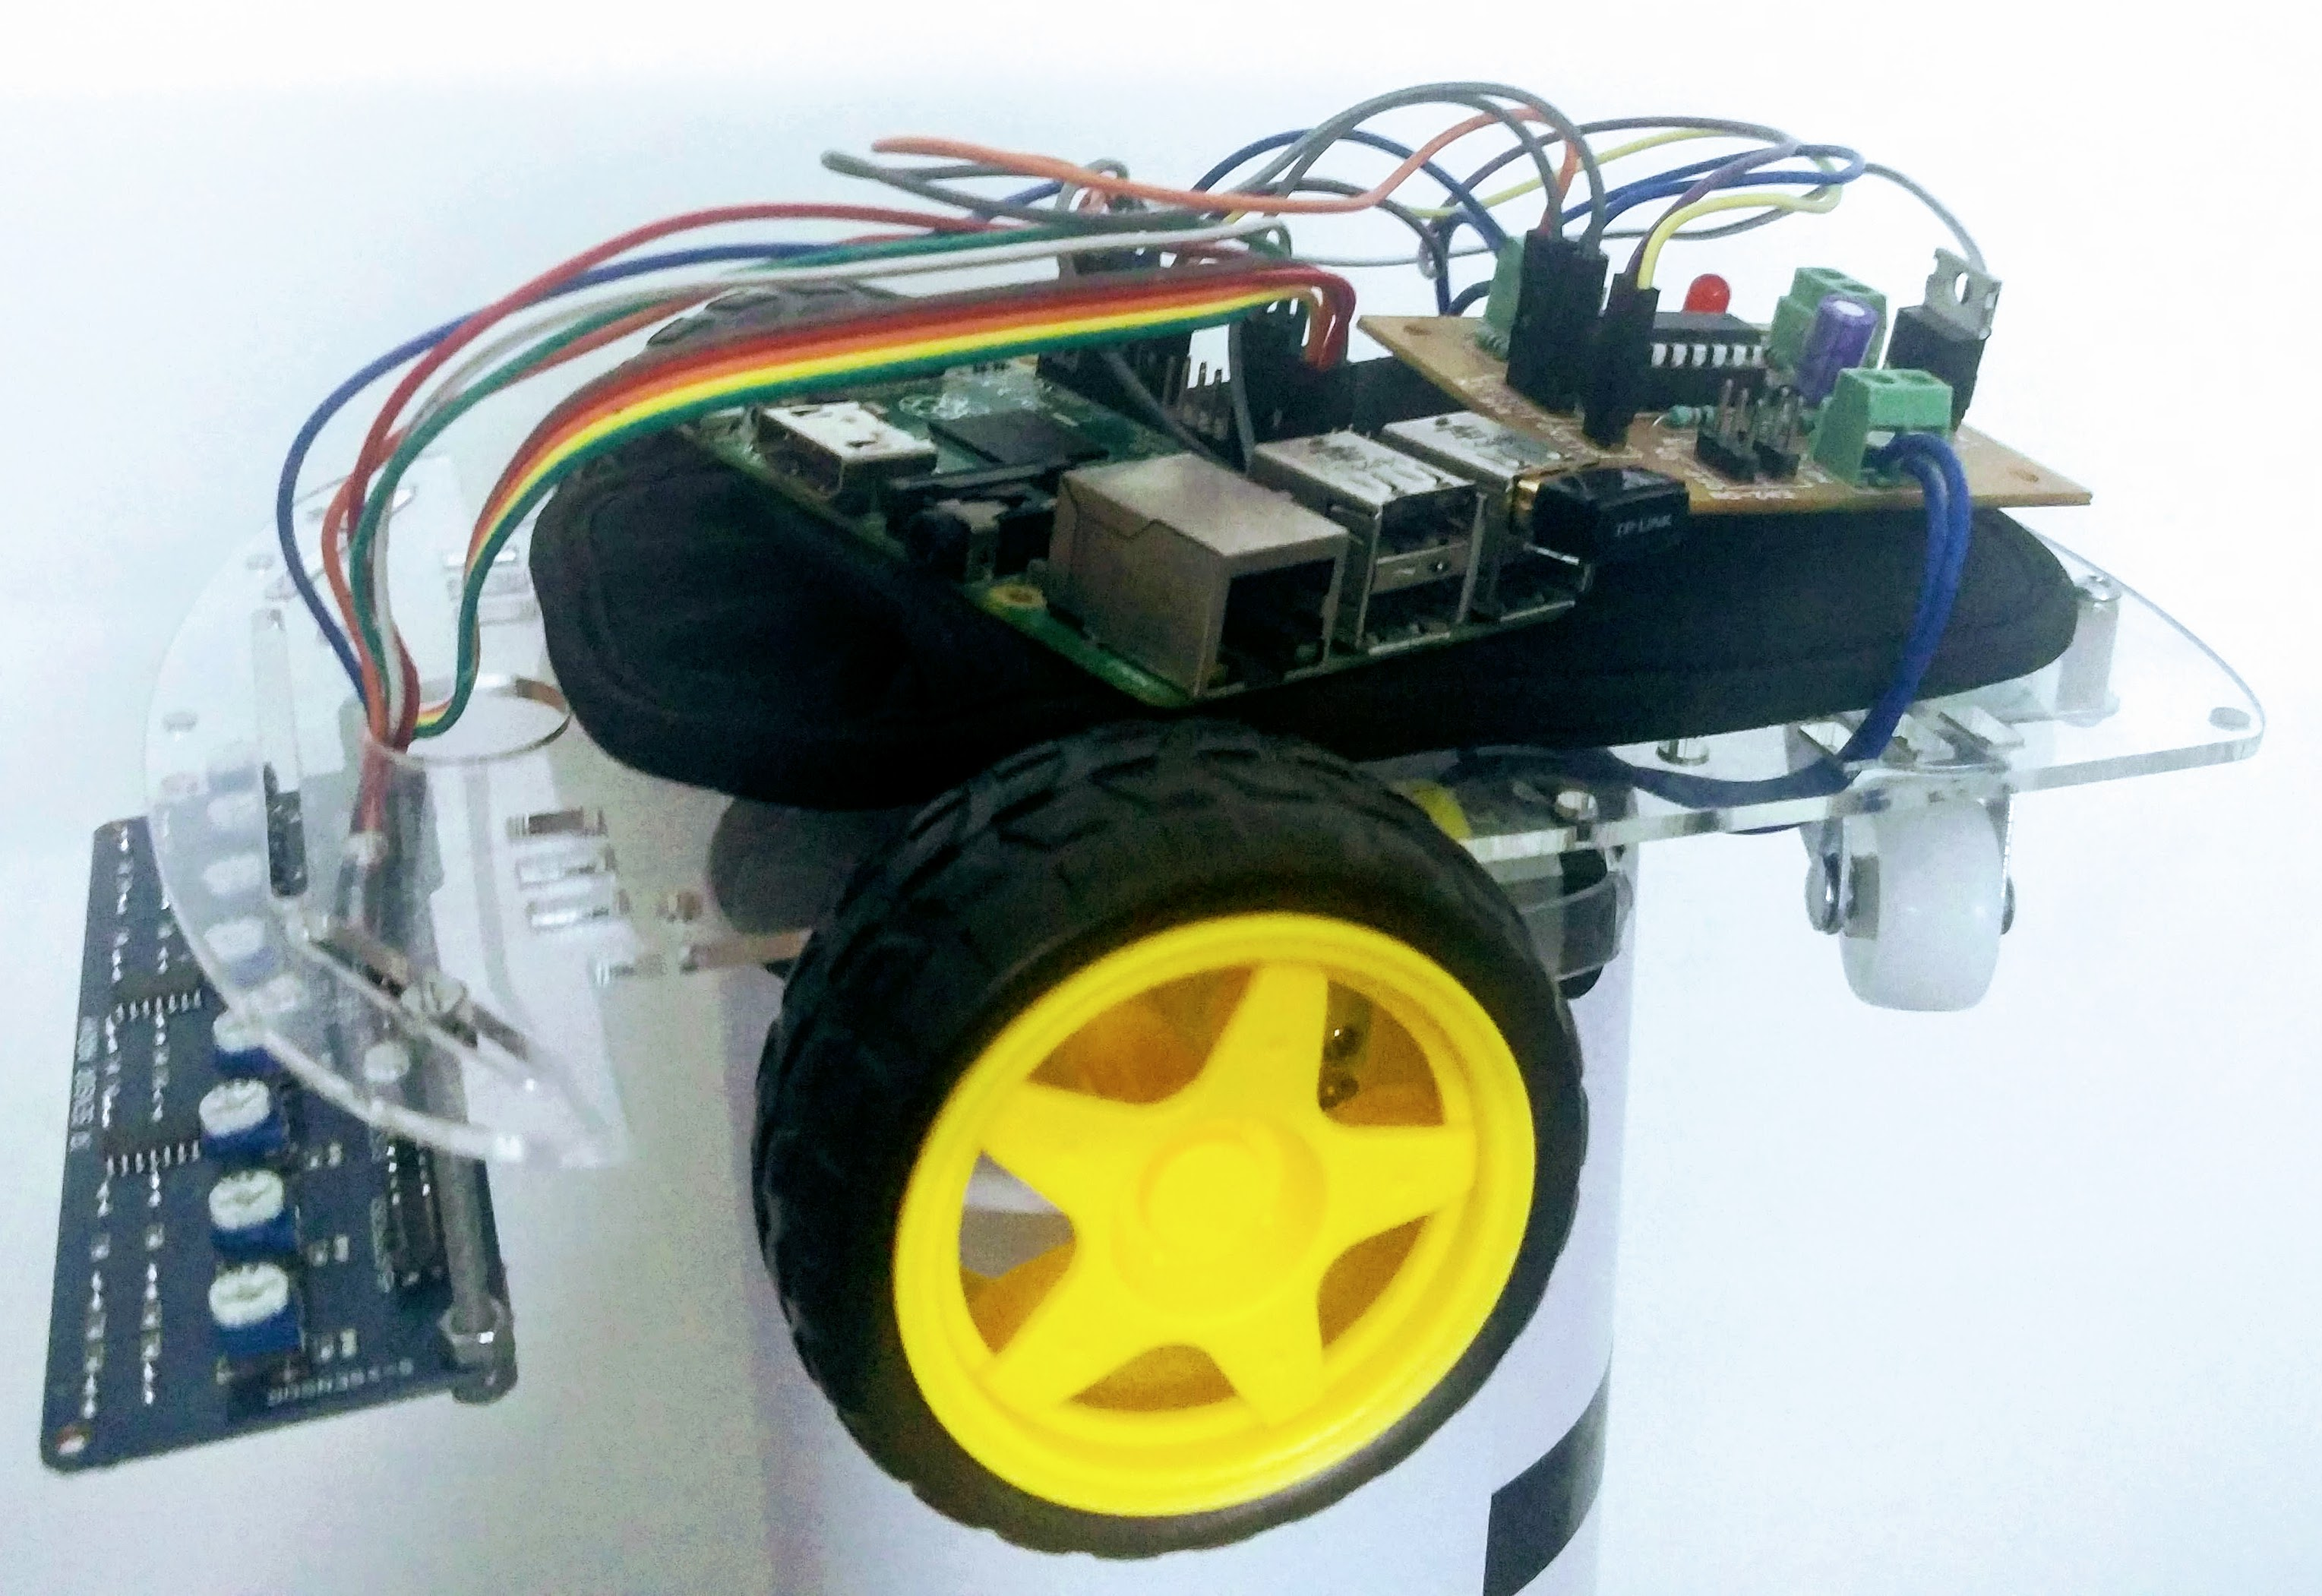
\includegraphics[width=\textwidth]{bot}
    \caption{Model Bot}
\end{figure}


\chapter{Algorithm}

\section{Reinforcement Learning}

Reinforcement Learning allows agents to automatically determine the ideal behaviour
 in order to maximize the performance. Environment provides the reward feedback
 required by the agent to learn its behaviour.

Markov Decision Process which is a discrete time stochastic control process are
typically used to model reinforcement learning problems. At each time step, the
process is in some state $ s $, and the agent may choose any action $ a $ that
is available in state $ s $ . The process responds at the next time step by
randomly moving into a new state $ s' $, and giving the agent a
corresponding reward $ R_{a}(s,s') $.

The probability that the process moves into its new state $ s' $ is
influenced by the chosen action. Specifically, it is given by the state transition
function $ P_{a}(s,s') $. Thus, the next state $ s' $
depends on the current state $ s $ and the agent's action $ a $.
But given $ s $ and $ a $, it is conditionally independent
of all previous states and actions; in other words, the state transitions of an
MDP satisfies the Markov property.

\begin{defn}
A state $ S_t $ is Markov if and only if,
$$ P[S_{t+1} | S_t] = P[S_{t+1} | S_1, ..., S_t] $$
\end{defn}


\section{Q-learning}

Reinforcement learning concerns itself with the long-term reward, not just
the immediate reward.

The long-term reward is learned when an agent interacts with an environment
through many trials and errors. An agent remembers the previous actions that
lead to dead ends. It also remembers the sequence of actions that
leads it higer rewards.

The value function $ Q $ returns the rewards associated with every state-action pair.
It is a representation of the long-term reward an agent would receive when
taking this action at this particular state, followed by taking the best path
possible afterward.

\begin{defn}
For a policy $ \pi $, Value function $ Q $ in a state $ s $ is calculated as,
$$ v_{\pi}(s) = E_{pi}[R_{t+1} + \gamma R_{t+2} + \gamma^2 R_{t+3} + ... | S_t = s] $$
\end{defn}

Q learning is a model free method where we try to approximate the value function
using value iteration updates. During each iteration we select the action greedily
from the learnt value and then update the value function using the actual reward.

\begin{center}
    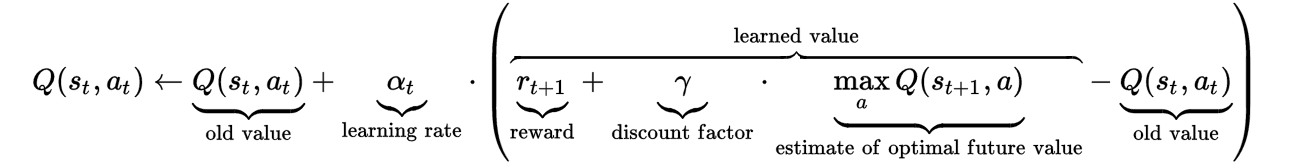
\includegraphics[width=\linewidth]{q0.png}
\end{center}

\begin{center}
    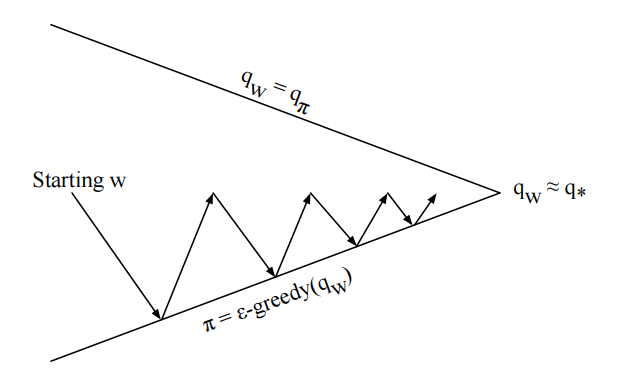
\includegraphics[width=0.8\linewidth]{q1.png}
    \captionof{figure}{Illustartion of value iteration methods approching optimal policy.}
\end{center}

\section{Deep Q-learning}

Neural networks can be effectively utilized to approximate the value function.
Using deep neural networks, value functions of problems with large number of
possible states can be predicated. Deep Q-learning has been used for solving
many challenging problem with staggering results.

Here is a pseudocode for the algorithm,

\begin{algorithm}
 \caption{Deep Q-learning}\label{q-learning}
 \begin{algorithmic}[1]
  \State Initialize action-value function Q with random weights
  \State Observe initial state s
  \For {episode = 1, M}
  \For {steps = 1, T}
  \State With probability select a random action $ a_t $
  \State Otherwise select $ a_t = max_a Q ∗ (\phi(s_t), a, \theta) $
  \State Execute action in emulator and observe reward $ r_t $ and image $ x_{t+1} $
  \State Set $ s_{t+1} = s_t, a_t, x_{t+1} $ and preprocess $ \phi_{t+1} = \phi(st+1) $
  \State $ y_j = r_j + \gamma max_{a'} Q(\phi_{j+1}, a'; \theta) $
  \State Perform a gradient descent step on $ (y_j - Q(\phi_j , a_j ; \theta))^2 $
  \EndFor
  \EndFor
 \end{algorithmic}
\end{algorithm}

\section{Neural Network Architecture}
The model used to train the simulation environment is three layers deep. All the three layers are dense, fully connected layers. The first layer accepts the raw inputs from the sensors of the bot, which are reshaped into an array of dimensions (1, 20), and then fed into the network. The subsequent hidden layer has neurons according to the task in hand. In a typical case, around 10 neurons work out to be fine. The final layer has neurons equal to the number of actions, which is three in our case.

We use ReLU activations for the input as well as hidden layers and softmax for the output layer. Adam is used as the optimization algorithm with cross-entropy loss.

\begin{figure}[htb]
    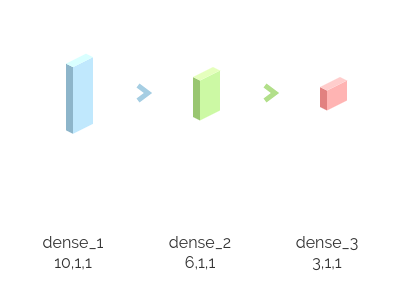
\includegraphics{net}
    \caption{Architecture of Neural Network}
\end{figure}

\chapter{Simulation} \label{simulation}

\section{The Need for Simulation} \label{need-for-simulation}
When a agent learns to perform actions using reinforcement learning, it
needs to interact with the environment. Though in principle it could
done using a physical robot, training a neural network on a physical bot posed
a lot of challenges.

\begin{itemize}
 \item The bot had to be placed on its starting position after every training episode. With more than 500 episodes to train, this would be cumbersome and impractical.
 \item Because of the minimum speed discussed in \autoref{testing-pretrained-models}, the bot would often run out of track, collide with barriers, or move in a random fashion. This should be avoided during training. In any such case, say, running out of the track, the bot can only return to the track by chance. The sensors would be ineffective, so there's no point in continuing that episode.
 \item Once the bot moved out of the chart paper on which the actual track was inscribed, it would receive abrupt inputs because of the rough surface beyond the chart paper. This would further hamper the learning process.
 \item In case of any of the above incidents, stopping the iteration manually involved a lot of latency. This uncertainity is not desired in the training process.
\end{itemize}

Hence, real-like simulations are essential to train and expirement with
algorithums. The simulation techniques we employed are discribed bellow.

\section{Simulation Techniques}
We used OpenAI gym as our primary interface the learning algorithm with the simulation envinorment. Initially we developed 2D simulations in Box2D and later a more robust system was developed using V-Rep.

\subsection{BOX2D}
Box2D is 2D simulation library in C++ with python bindings named as pybox2D. As pybox2D is part of the original OpenAI gym simulation environments, we developed a simulation for path follwing using OpenAI gym and pybox2D. This idea had a few major shortcomings which led to further improvisations and ultimately chucking the whole idea of pybox2D.

\begin{center}
    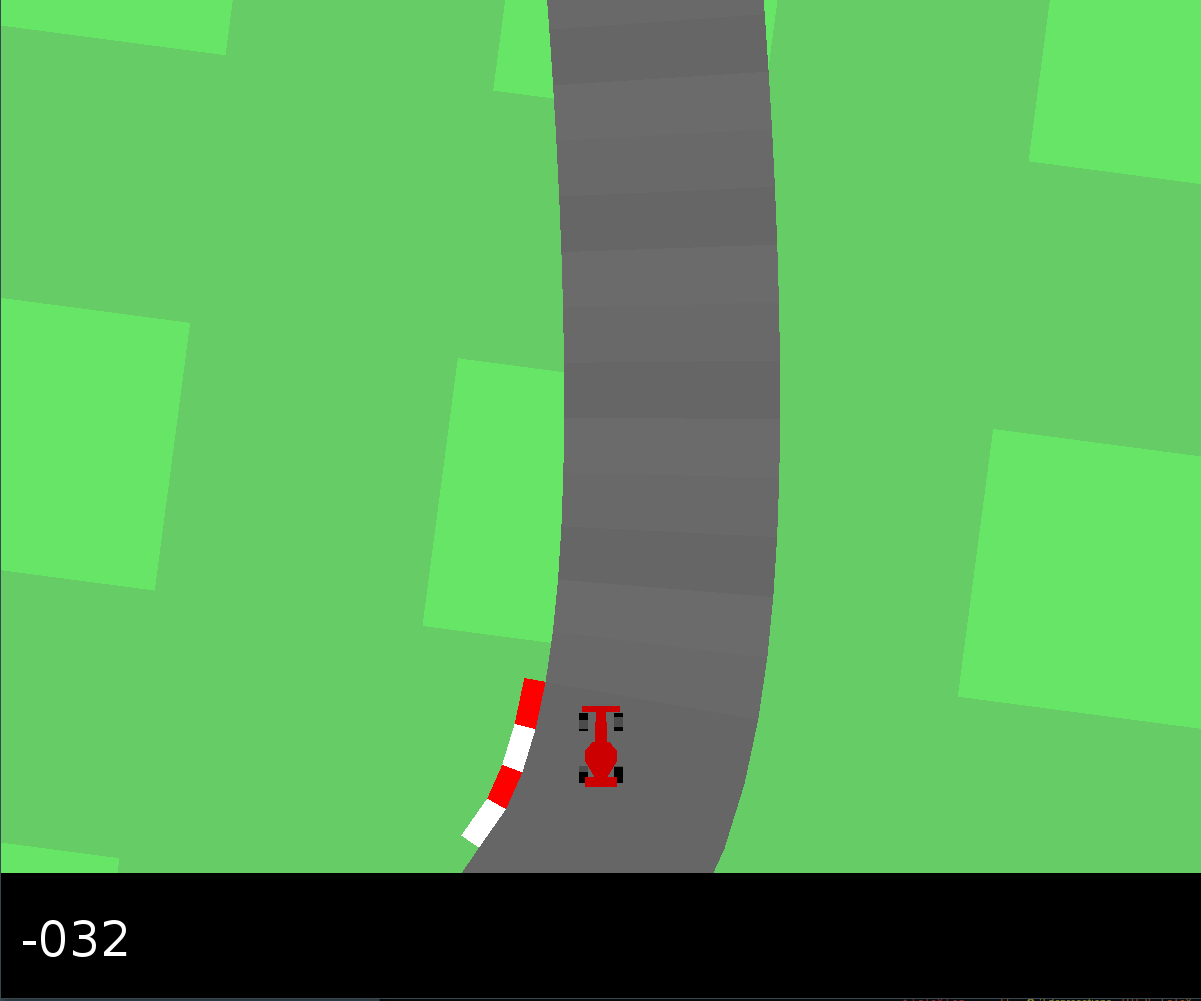
\includegraphics[width=0.8\linewidth]{1.png}
     \captionof{figure}{Path follwing simulation in Box2D.}
\end{center}

Particularly difficult was attaching ultrasonic sensors in the simulation. As the name suggests, this was a 2D simulation environment. Since our problem statement also included obstacle avoidance, we ultimately had to attach ultrasonic sensors on our simulation model. pybox2D didn't facilitate this very well.

\subsection{Gazebo}
Gazebo, \cite{gazebo} coupled along with ROS \cite{ros} is a very popular robot simulation software. We tried interfacing Gazebo with OpenAI gym based on \cite{gym-gazebo}, but could not get this getting to work in the first place. The installation procedure was quite cumbersome and required installing and compiling from various different sources. We faced a lot of problems while following the installation procedure, and ultimately decided to search for a different alternative.

\subsection{V-REP}
V-REP \cite{v-rep} is another simulation software similar to Gazebo, but with much simpler interface and easy integration with a variety of platforms, including python. This was relatively a piece of cake compared to installing Gazebo, and hence our choice when it comes to simulating a model bot. All of the simulation henceforth was carried out using V-REP

\begin{figure}[h]
    \centering
    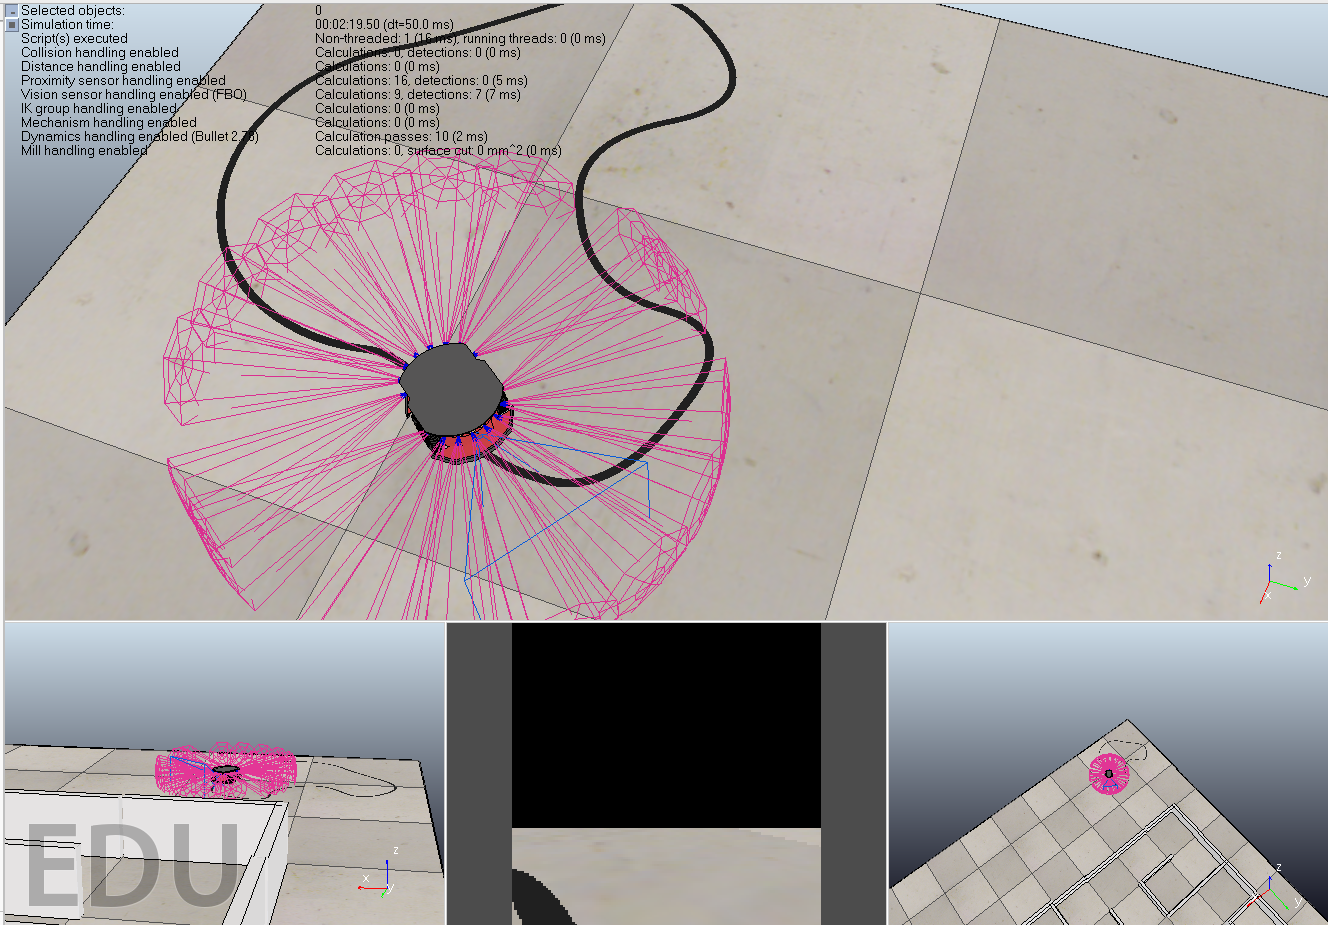
\includegraphics[width=0.8\linewidth]{2.png}
    \caption{Line follow simulation in V-Rep.}
\end{figure}

\begin{figure}[h]
    \centering
    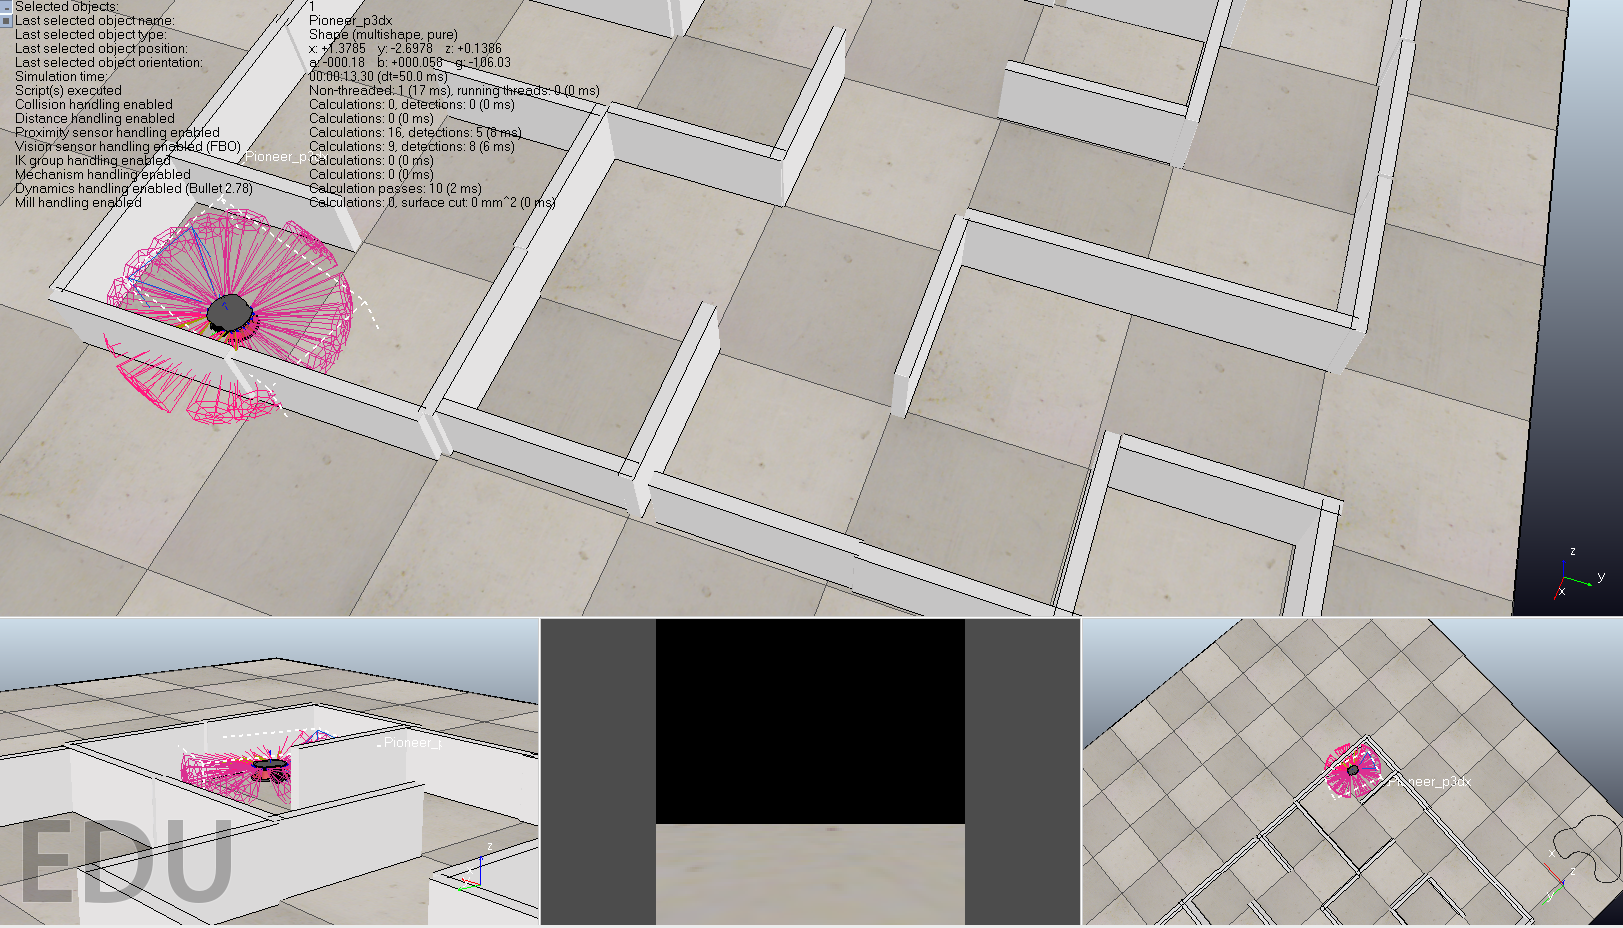
\includegraphics[width=0.8\linewidth]{3.png}
    \caption{Proximity sensor simulation in V-Rep.}
\end{figure}

\section{Training}

We used the already existing Pioneer 3DX model for our simulations. We first developed an interfacing script similar to OpenAI gym which lets us control the actual simulation from a python script. Next, we implemented the deep Q learning algorithm using keras with TensorFlow backend.

The training took well over 150 episodes with about 500 steps in each episode. The whole process took around 5 hours to complete. Initially the number of steps were limited to 100 to prevent the bot from exploring the track for the rest of the timesteps. This was then gradually increased as the bot started to learn in the initial few episodes.

This trained model was then used to run the physical model as described in \autoref{testing-pretrained-models}


\chapter{Physical Model}
The aim of this project was also to demonstrate the use of the algorithm in the real world. To serve this purpose, we built a physical model of a mobile robot using readily available components.

\section{Components}
The following major components were used in the physical model of the bot. Any relevant specifications are also listed below.

\begin{table}[h]
\centering
\begin{tabular}{@{}ll@{}}
\toprule
Component                       & Details           \\ \midrule
Acrylic Chassis                 & 2 Wheel Drive     \\
IR Sensor Array                 & 8 Channel         \\
LM293D Motor Driver board       & 7805 Power Supply \\
Ultrasonic Range Finder Modules & 4                 \\
Power Adapter                   & 9V                \\
Raspberry Pi 2                  & Model B (2014)    \\
Breadboard                      & 1                 \\
Jumper Wires                    & 20                \\ \bottomrule
\end{tabular}%
\caption{List of Components}
\end{table}

\begin{figure}
    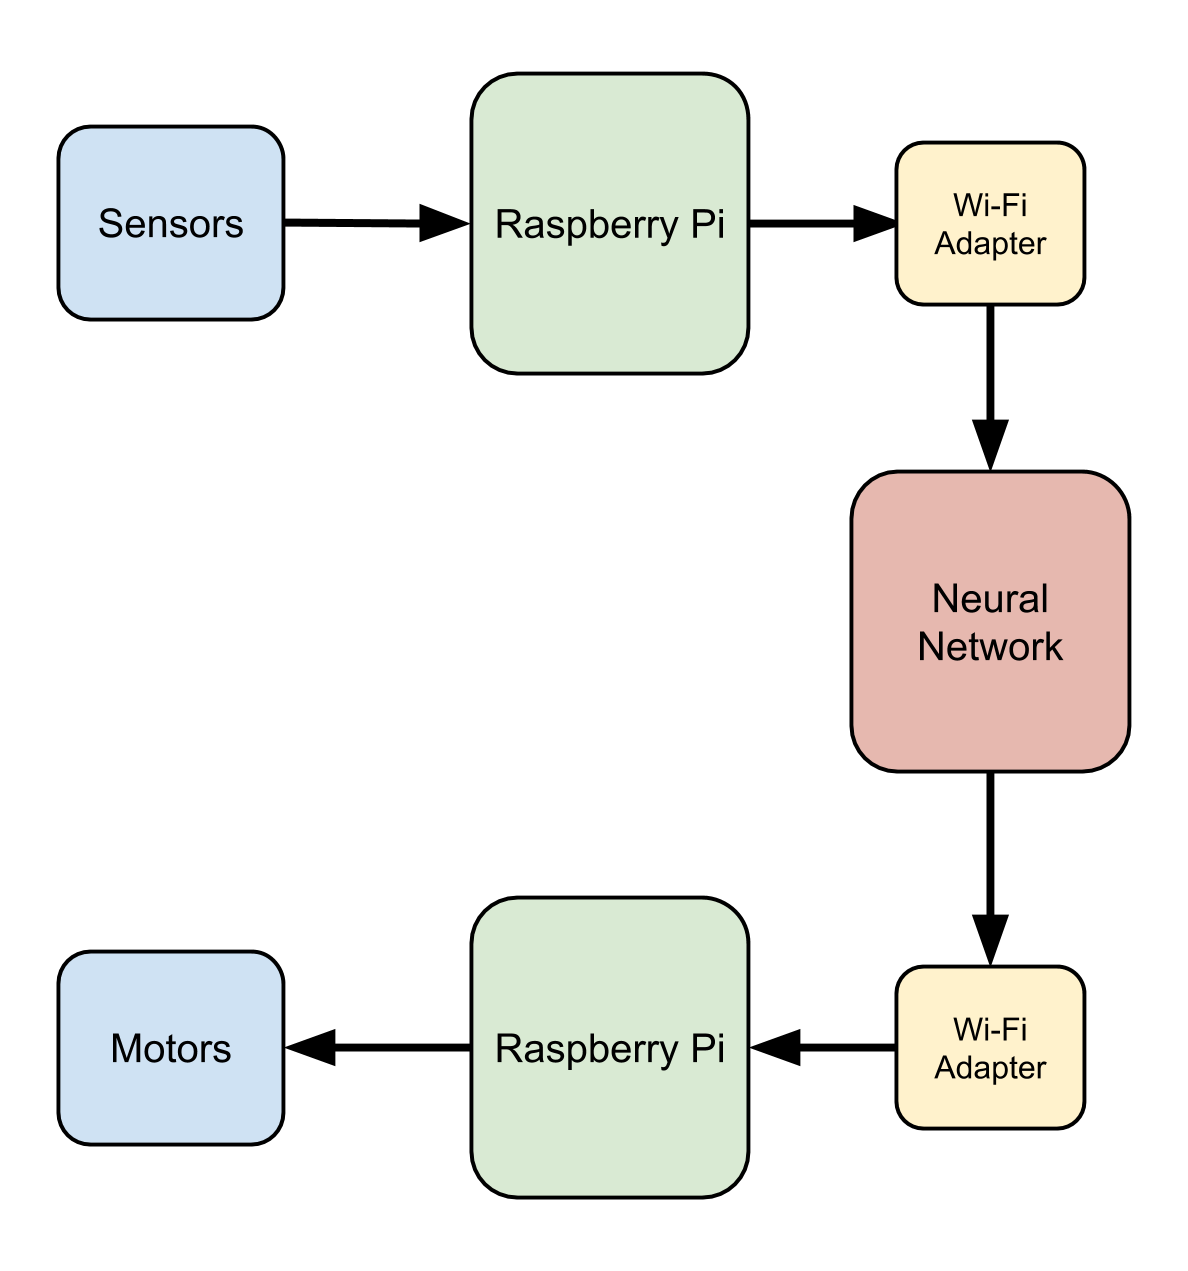
\includegraphics[width=\textwidth]{block}
    \caption{Block Diagram of one iteration of the control loop}
\end{figure}

\section{Microcontroller}
Both, the Raspberry Pi and the Arduino could be used as the microcontroller for the bot. But since the Raspberry Pi runs Python out of the box, it was the obvious choice when it comes to machine learning. Also, libraries such as TensorFlow are specially designed to run on Raspberry Pi. The specifications of the Raspberry Pi used are given below

\begin{table}[h]
\centering
\begin{tabular}{ll}
\toprule
Attribute     & Details             \\ \midrule
CPU           & BCM2836             \\
CPU Cores     & 4                   \\
CPU Speed     & 900 MHz             \\
RAM           & 1 GB                \\
Header Pins   & 40                  \\
Dimensions    & 3.35″ × 2.2″ × 0.8″ \\
Weight        & 42g                 \\
Rated Current & 800 mA              \\
Rated Voltage & 5 V                 \\ \bottomrule
\end{tabular}
\caption{Raspberry Pi 2 Model B Specifications}
\end{table}

\begin{figure}[h]
    \centering
    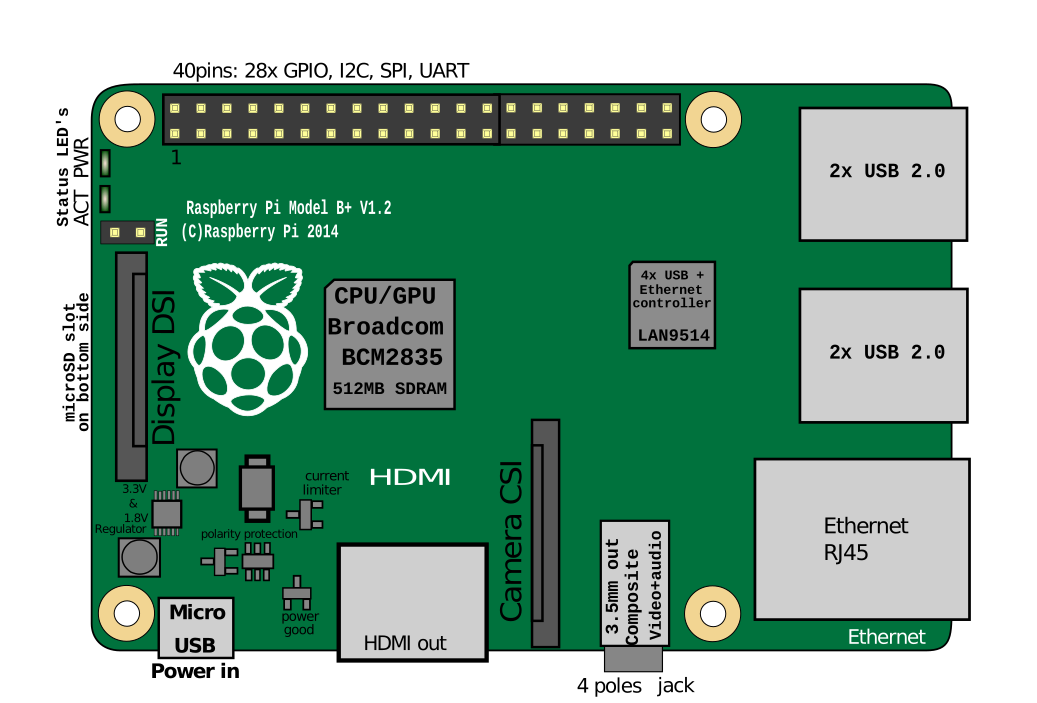
\includegraphics{rpi}
    \caption{Raspberry Pi 2 Model B}
\end{figure}

\section{Networking and Communications}
The Raspberry Pi on the bot was connected to a home WiFi network using an external WiFi adapter. Our computer was also connected to the same network.
An SSH server was enabled on the Pi which allowed accessing it remotely from the computer. All of the programs were uploaded using SSH.

Testing pretrained models trained in \autoref{simulation} on the bot had its own issues. The python script on the computer needed to communicate with the bot in order to get sensor values. We needed some form of interprocess communication, which was not possible natively using SSH.

\subsection{ZeroMQ}
We tried out ZeroMQ, the distributed messaging library. Although we were able to exchange close to 400 messages per second, we later realized that we also needed to provide the bot with actions computed by the network. This posed a problem because ZeroMQ uses a blocking queue. The communications would freeze very often on the occasion of frequent deadlocks.

\subsection{Flask}
HTTP was the next best available mode of communication and \texttt{Flask} was the next best tool for the purpose. Being lightweight, it did not hamper connection speed. Also, it runs quite well on the RPi. Since HTTP was built to support multiple channels and because it was non blocking, this solution worked quite well.

So we set up a \texttt{Flask} server on the RPi and used the \texttt{requests} package to send \texttt{POST} requests on the Flask server with actions, which, in turn, would return the observations of the sensors.

\section{Power}

The Raspberry Pi requires around 5V, which is a feeble amount of power and can easily be provided through USB devices. To facilitate portability, a USB Power Bank was used.

The motors, however, are a different story. Each of the motors had a specified power rating of 9V, 600mA, which cannot be powered from the same USB power source as that for the Pi. Thus, the motors required a different power source.

We initially tried powering with a standard 9V battery only to find out that it lasts only a few hours. In case the bot required training, this would be a terrible idea.

At last, we decided to use an external power adapter which converts utility power to 9V DC. This setup worked well for all experiments.

\section{Testing Pretrained Models} \label{testing-pretrained-models}
For the few experiments we performed while testing the pretrained models trained in \autoref{simulation}, the results suggested a few changes that needed to be made before achieving decent results. The following challenges were faced.

\begin{itemize}
 \item There was a considerable difference in the size of the actual track and the track used while simulation. We did not take into account this fact while making the simulation.
 \item The rate of acquiring observations in the real world was significantly faster than that from simulations. We believe this is because a sizeable chunk of the computer's resources were being used in simulation, resulting in slower data acquisition.
 \item The actual bot was considerably heavy and the motors didn't provide enough torque to move the bot at lower speeds. This resulted in a \emph{minimum speed} of the bot, below which it refulsed to move.
\end{itemize}

\section{Training Physical Model}

We wanted to avoid training a physical model at all costs due to reasons listed in \autoref{need-for-simulation}, but due to the unexpected outcomes in \autoref{testing-pretrained-models}, we tried this anyway. The following observations prove why training an actual model is a really terrible idea.

\begin{itemize}
    \item There was a mismatch of scale of the simulated model and the actual bot. In theory, we could run the bot at whatsoever speed we want provided it is between the operating limits, but it turns out that the sheer weight of the bot combined with a portable power source was large enough to create a minimum barrier speed that the bot could achieve. This \emph{minimum speed} was faster than actually required for efficient training. We eventually had to remove the portable power source and replace it with a wired one.
    \item In the initial phase of training, the bot is biased about the actions it needs to take. Since we had four actions, all of them were equally probable. During our experiments, the bot almost chose to take left turns, which led to the different cords (introduced due to excessive weight) being used to tangle. In only one minute of training, the process had to be stopped for this very reason.
    \item The bias for a particular action was further reinforced when the bot actually got positive rewards when it reached the end of the track and could not move. This was clearly not desired, and further justified the need for simulation.
    \item The reward function was then modified and made biased to give better rewards to move forward, but this in turn made learning other actions really difficult.
\end{itemize}

All of these practical difficulties further testify the requirement of simulations. Reinforcement learning problems on physical models are better done through transfer learning with better choice of simulation parameters as to match with the physical implementation of the physical model.

\chapter{Conclusions}
In this project, we aimed to test out the recently popular reinforcement learning paradigm which can be easily adapted to tasks like robot locomotion. This project led to the following conclusions.

\begin{itemize}
    \item We were successful in implementing the Q learning algorithm in simulation, which was able to train in a relatively short span of around 150 episodes. This further strengthens the applicability of reinforcement learning to such tasks, and shows that we are headed in the right direction.
    \item We developed an interface to the popular Pioneer 3DX bot available for V-REP. The bot can now be fully controlled via python. This is an added contribution to the open source community.
    \item We discovered that algorithms such as reinforcement learning which require training for extended periods have to be accompanied by simulation. Performing the training process on an actual bot poses a lot of challenges.

\end{itemize}

\chapter{Future Directions}

The original idea of the project was to develop an algorithm for autonomous robots in a controlled enviromnent such as that of a warehouse. Our implementation was able to learn the basic path following algorithm successfully, but a lot of the ideas of the original problem statement remain to be executed. Some of them include

\begin{itemize}
    \item Incorporating ultrasound sensors efficiently into the learning algorithm, so the bot also learns to avoid obstacles apart from following a predefined path.
    \item Developing mechanisms for localization. This could be implemented by identifying landmarks in the path, such as intersections, and then trying to locate the current position of the bot.
    \item Ability to interface other algorithms such as identifying the shortest path along with the core Q learning algorithm. This would facilitate greater control over the otherwise autonomous bot.
    \item Better control of locomotion through more fine tuned controls for motor speeds. This would enable the bot to not only traverse flat surfaces, but also move efficiently in uneven terrains.
\end{itemize}


\bibliographystyle{apalike}
\bibliography{references}

\end{document}
